
\begin{figure}
    \centering
    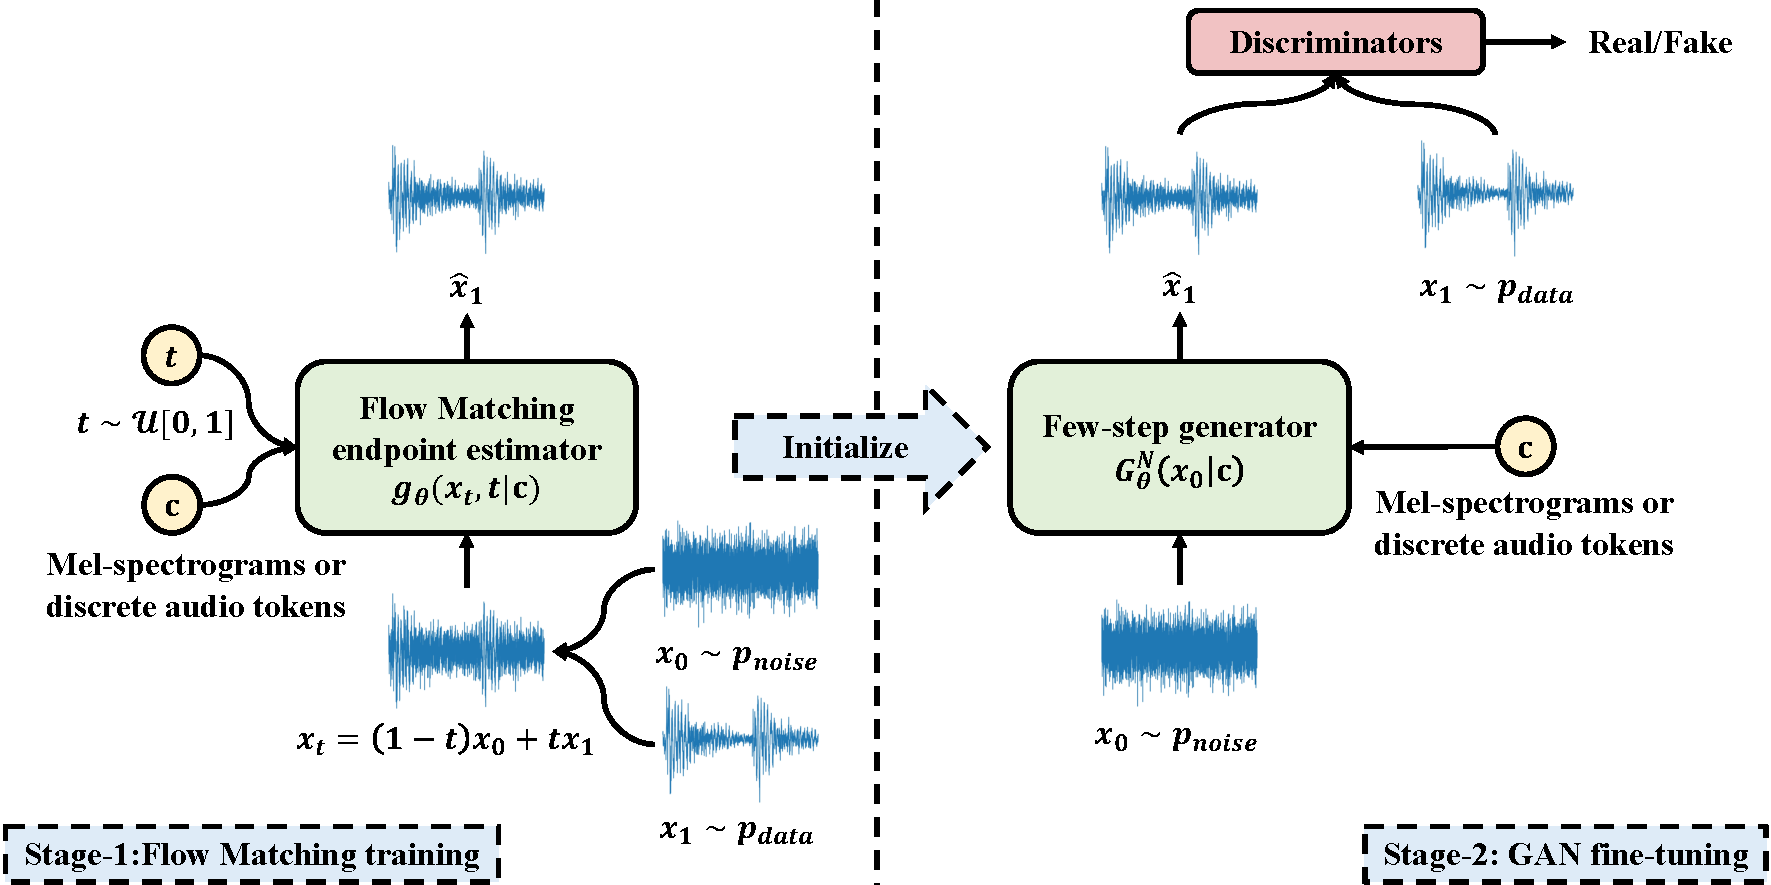
\includegraphics[width=0.8\linewidth]{fig/framework}
    \vspace{-0.6em}
	  \caption{Overall framework of Flow2GAN.}
	\label{fig:framework}
    \vspace{-1.8em}
\end{figure}

As illustrated in Figure~\ref{fig:framework}, Flow2GAN follows a two-stage training strategy: the model is first trained with improved Flow Matching tailored for audio modeling (Section~\ref{ssec:improved_fm}); then few-step generators are built with the trained model and guided by GAN fine-tuning toward fine-grained generation (Section~\ref{ssec:gan_ft}). The model utilizes a multi-branch architecture that processes Fourier coefficients at different time-frequency resolutions (Section~\ref{ssec:multi-branch}).  

\vspace{-0.8em}
\subsection{Improved Flow Matching for audio modeling}
\label{ssec:improved_fm}
\vspace{-0.5em}

\begin{figure}
    \centering
    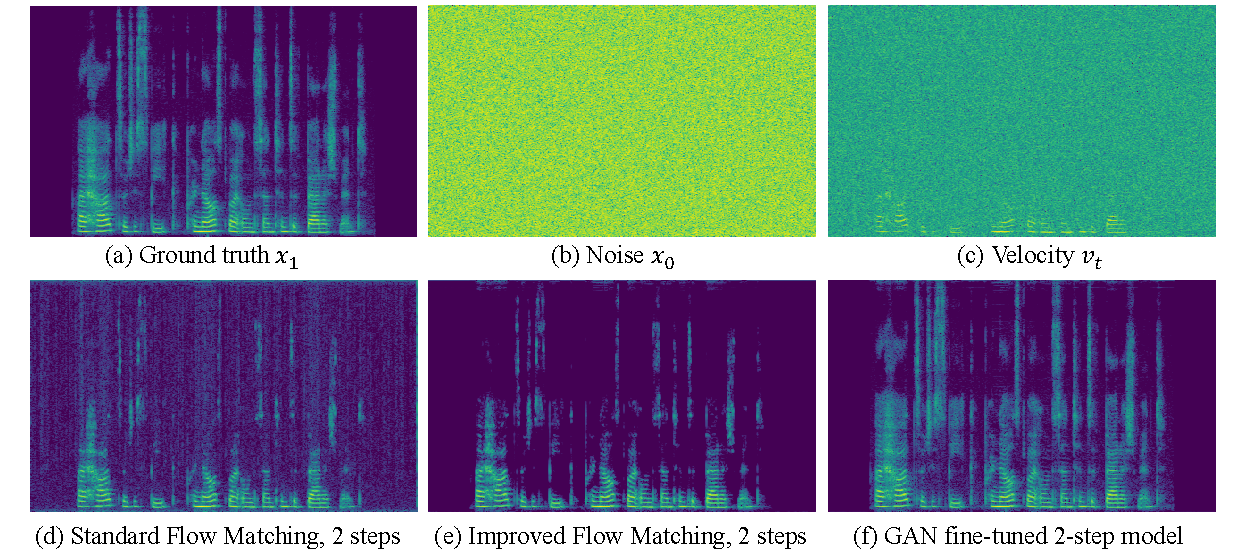
\includegraphics[width=0.8\linewidth]{fig/fm_sample}
    \vspace{-0.8em}
	  \caption{Example illustration of audio generation. Flow Matching estimates velocity $v_t=x_1-x_0$. The improved Flow Matching in Flow2GAN estimates endpoint $x_1$, yielding cleaner result in silent regions with 2 sampling steps. GAN fine-tuning further enhances the result by filling in details.}
	\label{fig:fm_sample}
    \vspace{-1em}
\end{figure}

% \yao{we focus on one-/two-step flow}

When applying Flow Matching to conditional audio generation, the velocity field is parameterized as $f_{\theta}(x_t, t|\mathbf{c})$, where $\mathbf{c}$ denotes the compressed acoustic representations, such as Mel-spectrograms or discrete audio tokens. 
% We argue that, due to the unique characteristics of audio data (see figure~\ref{}), employing Flow Matching in this setting involves two main challenges:
However, the unique characteristics of audio data present two key challenges for Flow Matching in this context: 1) \textbf{Velocity estimation difficulty.} Audio signals often contain silent segments or frequency bands with zero energy (Figure~\ref{fig:fm_sample} (a)). In these regions, the model must accurately estimate $v_t$ to precisely cancel out the noise in $x_0$ and recover the empty target $x_1$. This increases the learning difficulty as the model is required not only to capture the differences $v_t = x_1 - x_0$ in the active regions of the audio signal, but also to approximate $-x_0$ in these empty regions (Figure~\ref{fig:fm_sample} (c)). 
2) \textbf{Loss-perception mismatch.} The Flow Matching loss (Equation~\ref{eq:fm_loss}) uses mean squared error (MSE) criterion, treating the prediction errors uniformly across all signal regions. However, this does not align well with auditory perception principles, where errors in quieter spectral regions tend to be more perceptually noticeable than equivalent errors in louder regions. 

\vspace{-0.1em}
\noindent\textbf{Reformulation to endpoint estimation.} To circumvent
the difficulty of predicting the velocity $v_t$, we reformulate the Flow Matching problem so that the network predicts the endpoint $x_1$ instead: $\hat{x}_1 =g_{\theta}(x_t, t|\mathbf{c})$. 
Specifically, as $v_t = \frac{x_1 - x_t}{1 - t}$, the loss in Equation~\ref{eq:fm_loss} can be rewritten as: 
\begin{equation}
\label{eq:fm_loss_x1}
\vspace{-0.2em}
\mathcal{L}_{\mathrm{FM}}
= \mathbb{E}_{t,x_0,x_1} \left[\left\| \frac{g_{\theta}(x_t, t|\mathbf{c}) - x_t}{1 - t} - \frac{x_1 - x_t}{1 - t} \right\|^2 \right]
= \mathbb{E}_{t,x_0,x_1} \left[\frac{\left\|g_{\theta}(x_t, t|\mathbf{c}) - x_1 \right\|^2}{(1 - t)^2}\right].
\vspace{-0.1em}
\end{equation}
This reformulation can be interpreted as training the network to reconstruct the clean audio $x_1$ from its noisy version $x_t$ at varying noise levels $(1-t)$. This approach provides a more consistent and stable learning objective tailored to audio data, allowing the network to focus on capturing audio-relevant patterns regardless of whether the region is active or empty. 
% The weighting factor $\frac{1}{(1 - t)^2}$ in Equation~\ref{eq:fm_loss_x1} assigns greater emphasis on instances where $x_t$ is closer to $x_1$. 
Empirically, we found that removing the weighting factor $\frac{1}{(1 - t)^2}$ in Equation~\ref{eq:fm_loss_x1} yields slight improvements at both the Flow-Matching stage (2 steps) and after GAN fine-tuning. The reason might be that without this weighting, the model can better emphasize small $t$ values, which aligns well with our setting.
% Empirically, we found that removing this factor leads to a slight performance degradation in the Flow Matching training stage, but this gap vanishes after GAN fine-tuning (Section~\ref{ssec:gan_ft}) \yao{(even slightly better, no drop at 2 step)}. 
For simplicity, we therefore omit this factor, yielding:
\begin{equation}
\label{eq:fm_loss_x1_no_scale}
\vspace{-0.2em}
\mathcal{L}_{\mathrm{FM}}' 
= \mathbb{E}_{t,x_0,x_1} \left[\left\|g_{\theta}(x_t, t|\mathbf{c}) - x_1 \right\|^2\right].
\vspace{-0.2em}
\end{equation}
%\footnote{In our experiments, we clamp the loss weight $\frac{1}{(1 - t)^2}$ to a maximum of 100.0 for training stability.}.
The sampling process in Equation~\ref{eq:fm_ode} is consequently modified as follows: 
\begin{equation}
\label{eq:fm_ode_x1}
\vspace{-0.3em}
x_{t_{i+1}} = x_{t_i} + (t_{i+1} - t_i)\frac{g_{\theta}(x_{t_i}, t_i|\mathbf{c}) - x_{t_i}}{1 - t_i}.
\vspace{-0.3em}
\end{equation}

\noindent\textbf{Spectral energy-adaptive loss scaling.} To address the loss-perception mismatch, we scale the Flow Matching loss inversely proportional to the energy of the reference spectrogram, thereby encouraging the model to emphasize the perceptually salient quieter regions. Specifically, the prediction error is converted into frequency domain: $\mathcal{S}(g_{\theta}(x_t, t|\mathbf{c}) - x_1)$, where $\mathcal{S}(x)=\mathrm{LinFB}(|\mathrm{STFT}(x)|^2)$ denotes the power STFT followed by a linear filterbank transformation for energy smoothing, and is differentiable. The obtained result is then scaled element-wise inversely by the square root of the reference spectrogram’s energy, $\frac{1}{\sqrt{\mathcal{S}(x_1) + \epsilon}}$, with $\epsilon=1e-7$. Therefore, the loss in Equation~\ref{eq:fm_loss_x1_no_scale} is redefined as:
\begin{equation}
\label{eq:fm_loss_x1_scaling}
\vspace{-0.2em}
\mathcal{L}_{\mathrm{FM}}''
= \mathbb{E}_{t,x_0,x_1} \left[ \sum_{i,j} 
\left(\frac{\mathcal{S}(g_{\theta}(x_t, t|\mathbf{c}) - x_1)}{\sqrt{\mathcal{S}(x_1) + \epsilon}}\right)_{i,j} \right].
% \vspace{-0.2em}
\end{equation}
We clamp the loss scale $\frac{1}{\sqrt{\mathcal{S}(x_1) + \epsilon}}$ between 0.01 and 100 for training stability. See Appendix Table~\ref{tab:model_conf} for detailed configurations of $\mathcal{S}(x)$. 
Note that unlike the per-frame energy-based scaling in previous works~\citep{priorgrad,rfwave}, our scaling strategy is more comprehensive as it also accounts for differences along the frequency dimension.

% We believe the target x_1 might "easier" for the network to learn to output than the velocity x_1 - x_0 because in parts of time-frequency space where x_1 is quiet, the velocity x_1 - x_0 would not necessarily be quiet, yet the process of computing x_1 from (t, x_t and v_t) involves cancellation of the noise in x_0; this would require a very precise estimate of v_t to do accurately as we are predicting a quiet thing from a difference of two loud things.  There is a linear relationship between v_t and x_1, assuming t and x_t are known.  Thus, when we change the target from v_t to x_1 we can view it as being a reformulation of the problem, fundamentally differing only in having a different "t"-dependent weighting of the loss.

% related works: PeriodWave, with discrete wavelet transformation; MBD, EQ

% \vspace{-2em}
\subsection{GAN Fine-tuning for Refinement and Few-step Inference}
\label{ssec:gan_ft}
% \vspace{-0.8em}

% Although the adaptations described in Section~\ref{ssec:improved_fm} improve the audio generation quality of the Flow Matching model with 2 sampling steps (see Figure~\ref{fig:fm_sample} from (d) to (e) and Table~\ref{tab:ablation_flow}), the inherent complexity of audio generation still leaves room for further refinement. 
Although the adaptations described in Section~\ref{ssec:improved_fm} improve the audio generation quality of the Flow Matching model with 2 sampling steps (see Figure~\ref{fig:fm_sample} (d) to (e) and Table~\ref{tab:ablation_flow}), the inherent complexity of audio generation still leaves room for further refinement of details, especially in the high-frequency range. 
Moreover, even though we can obtain higher quality results through multi-step sampling (see Table~\ref{tab:ablation_multi_step} in Appendix), this would require considerable computational overhead. To this end, we employ a GAN fine-tuning strategy for two purposes: enhancing the fine-grained audio details by leveraging the existing carefully designed discriminators~\citep{hifigan, mrd} that capture diverse audio patterns from multiple perspectives, and enabling high-fidelity generation with few-step (even only one-step) inference. 

% We construct the one-step and two-step GAN generators, referred to as $G_{\theta}^1(x_0|\mathbf{c})$ and $G_{\theta}^2(x_0|\mathbf{c})$, by forwarding the trained Flow Matching model through the corresponding number of steps: $G_{\theta}^1(x_0|\mathbf{c})=g_{\theta}(x_0,0|\mathbf{c})$, and $G_{\theta}^2(x_0|\mathbf{c})=g_{\theta}(\frac{x_0 + g_{\theta}(x_0, 0|\mathbf{c})}{2},0.5|\mathbf{c})$. 
We construct the few-step GAN generators, referred to as $G_{\theta}^N(x_0|\mathbf{c})$, by forwarding the trained Flow Matching model through $N$ steps following Equation~\ref{eq:fm_ode_x1}. 
Note that generators with different steps are trained and deployed as separate models rather than a single unified model.
Specifically, for $G_{\theta}^N(x_0|\mathbf{c})$ with $N>1$, gradients are backpropagated through both forward passes, enabling end-to-end optimization of the intermediate output from earlier steps. While this approach can extend to more steps, we focus on one-, two-, and four-step variants for computational efficiency. Following~\citep{vocos}, we adopt the multi-period discriminator (MPD)~\citep{hifigan} and the multi-resolution discriminator (MRD)~\citep{mrd} for adversarial training. The generators are fine-tuned using a combination of HingeGAN adversarial loss~\citep{hingegan}, $L1$ feature matching loss, and multi-scale $L1$ Mel-spectrogram reconstruction loss~\citep{dac}. 

% \yao{Detailed loss scales}.

We found that a fast stage of GAN fine-tuning is sufficient to yield a rapid and substantial improvement in audio quality, while additional fine-tuning can provide further gains (see  Table~\ref{tab:ablation_gan}). Figure~\ref{fig:fm_sample} (e) to (f) shows that the fine-grained details are recovered after GAN fine-tuning. Intuitively, this effect arises because the pre-training stage with the improved Flow Matching objective already equips the model with strong generative modeling capabilities, while subsequent fine-tuning efficiently guides the model toward high-fidelity output by iteratively refining details through adversarial learning with real audio samples. 
As shown in Table~\ref{tab:ablation_flow}, it is worth noting that when using standard Flow Matching for pre-training like~\citep{periodwave_turbo}, the one-step model achieves significantly lower performance after GAN fine-tuning, demonstrating the superiority of our improved Flow Matching objective.
This strategy combines the strengths of both paradigms - improved Flow Matching for robust generative capability learning, and GAN for detail enhancement - ultimately enabling high-fidelity audio generation with fast inference. Notably, compared to pure GAN training, it also requires significantly lower training cost.
 % and mitigates the risk of mode collapsing~\citep{gan,gan_collapse}.

% \vspace{-1em}
\subsection{Multi-resolution network structure}
\label{ssec:multi-branch}
% \vspace{-1em}

\begin{figure}
    \centering
    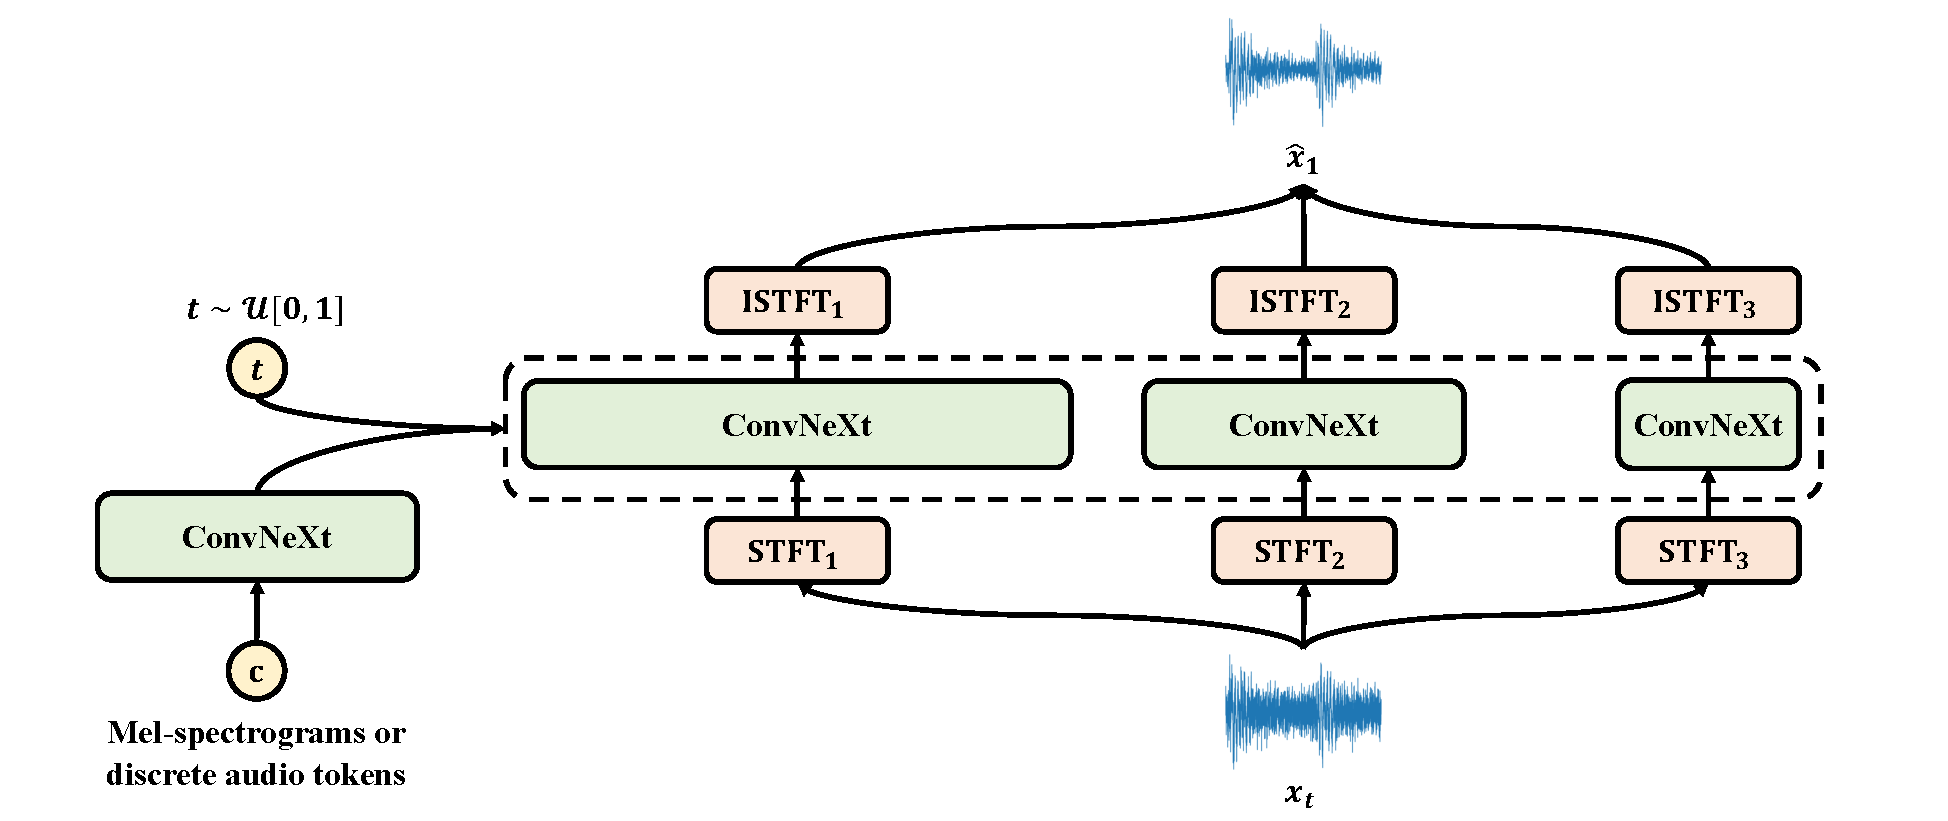
\includegraphics[width=0.9\linewidth]{fig/network}
    \vspace{-0.5em}
	  \caption{Multi-resolution network structure. Our model processes spectral coefficients from STFT at three different time-frequency resolutions, using larger embedding dimensions for shorter sequences. A ConvNeXt-based encoder processes the conditional compressed representation.}
	\label{fig:network}
    \vspace{-1.7em}
\end{figure}

Inspired by Vocos~\citep{vocos}, our model processes Fourier coefficients rather than waveform samples for saving computational cost and memory usage. While Vocos operates at a single time-frequency resolution, we extend to multi-resolution modeling to better capture audio complexity, providing a more powerful backbone for generative learning.

As shown in Figure~\ref{fig:network}, our model comprises three branches, each processing Fourier coefficients at different resolutions. Specifically, in each branch, the input signal is first transformed via STFT to obtain complex Fourier coefficients, whose real and imaginary components are concatenated along the feature dimension and fed into a ConvNeXT model~\citep{convnext} to produce output complex coefficients. These are then converted back to waveform domain via Inverse STFT (ISTFT). The final output is obtained by summing all branch outputs. Since both STFT and ISTFT operations are differentiable, the entire model is optimized end-to-end. Additionally, following~\citep{periodwave}, we incorporate a ConvNeXt-based condition encoder to extract deeper features from input Mel-spectrograms or codec token embeddings, which serve as shared generation conditions across all branches. Note that for Flow Matching inference, this condition encoder requires only one forward pass, with output features reused across multiple sampling steps. To better balance performance and efficiency, we use larger embedding dimensions for the low-frame-rate branch, and smaller embedding dimensions for the two high-frame-rate branches. Detailed model configurations are provided in Appendix~\ref{tab:model_conf}.  

% \yao{should: add block in Appendix}







